%
% Documento: Apêndice
%

\begin{apendicesenv}
\partapendices

\chapter{Resultados Catálogo selec20}
\label{chap:apendiceselec20}
Com a aplicação do nosso método nos 20 aglomerados do catálogo selec20 obtivemos os seguintes resultados, dado o histograma de velocidade, o eixo principal e o perfil de rotação apenas para os aglomerados que apresentaram rotação significativa.  

\begin{figure}[H] %h or !htbp
\vspace{-2pt}
\centering
\subfloat{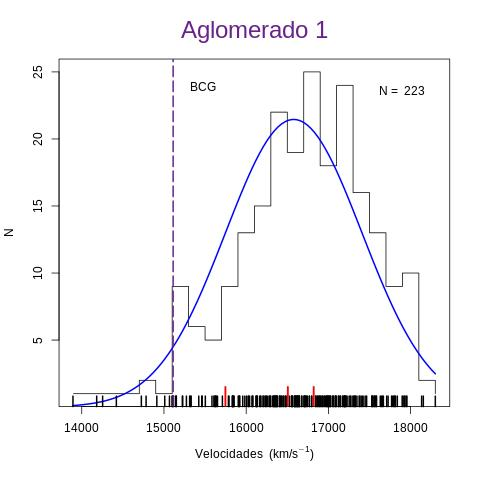
\includegraphics[scale=.23]{04-figuras/selec20//dist01}}
\subfloat{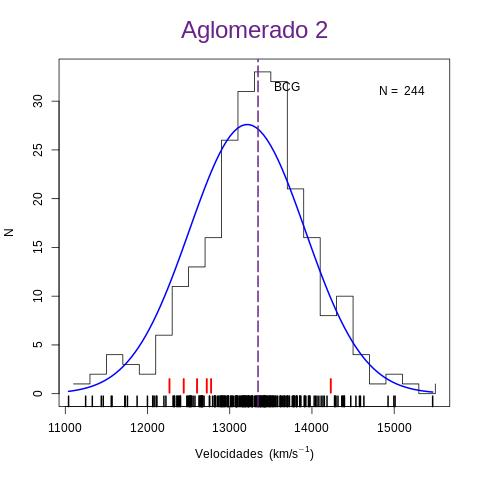
\includegraphics[scale=.23]{04-figuras/selec20//dist02}}
\subfloat{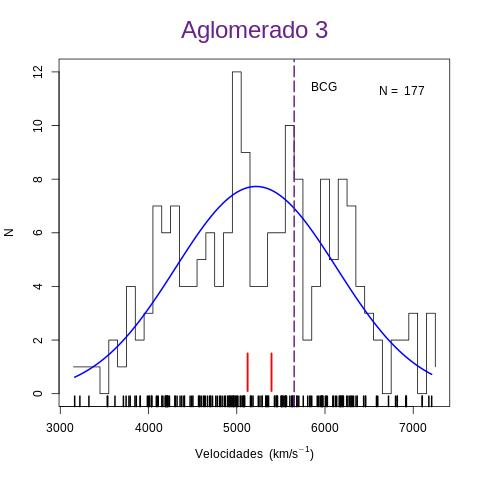
\includegraphics[scale=.23]{04-figuras/selec20//dist03}}
\subfloat{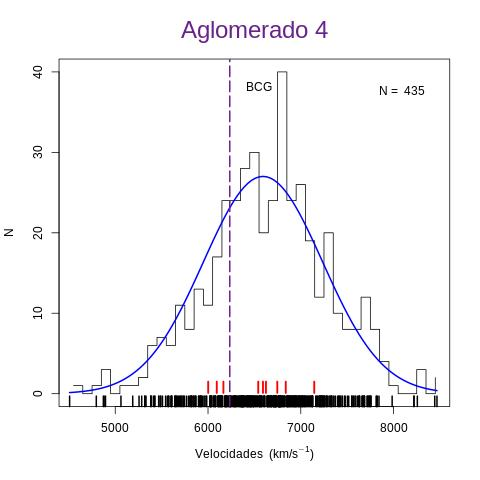
\includegraphics[scale=.23]{04-figuras/selec20//dist04}}\hfill
\subfloat{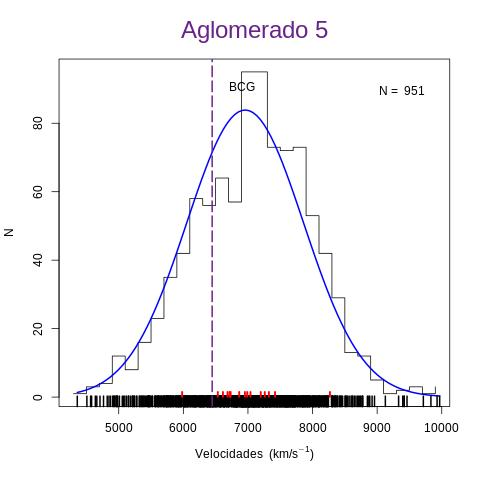
\includegraphics[scale=.23]{04-figuras/selec20/dist05}}
\subfloat{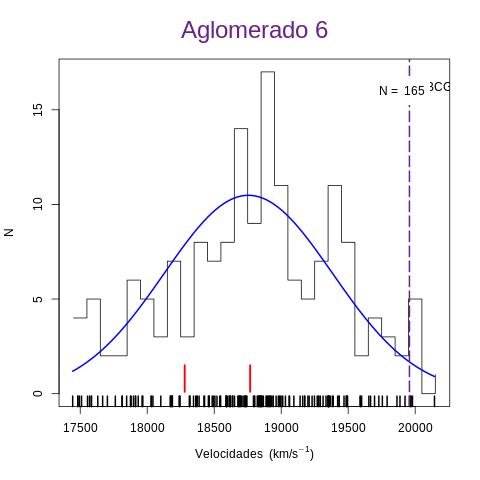
\includegraphics[scale=.23]{04-figuras/selec20/dist06}}
\subfloat{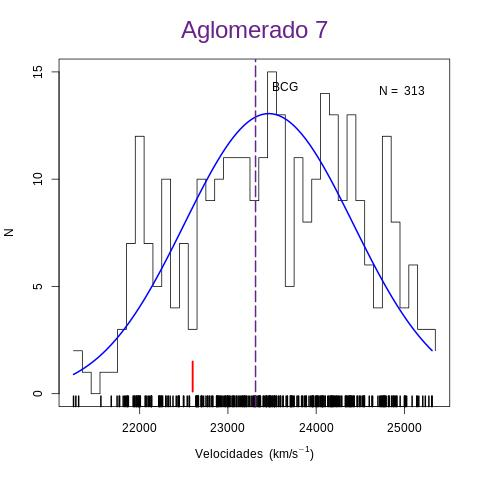
\includegraphics[scale=.23]{04-figuras/selec20/dist07}}
\subfloat{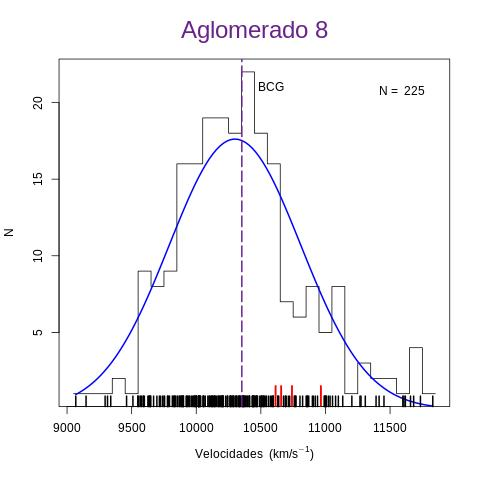
\includegraphics[scale=.23]{04-figuras/selec20/dist08}}\hfill
\subfloat{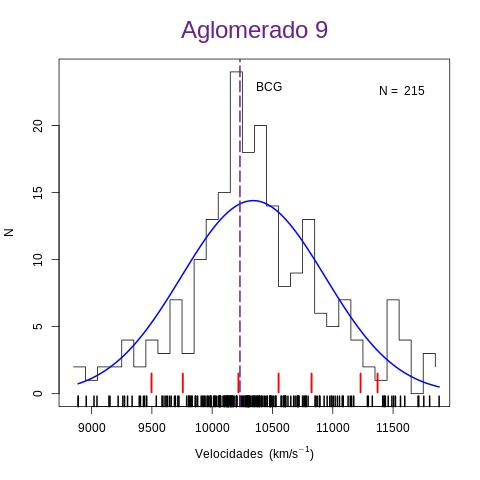
\includegraphics[scale=.23]{04-figuras/selec20/dist09}}
\subfloat{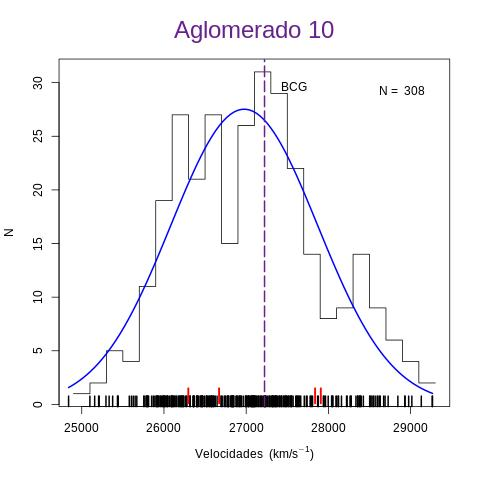
\includegraphics[scale=.23]{04-figuras/selec20/dist10}}
\subfloat{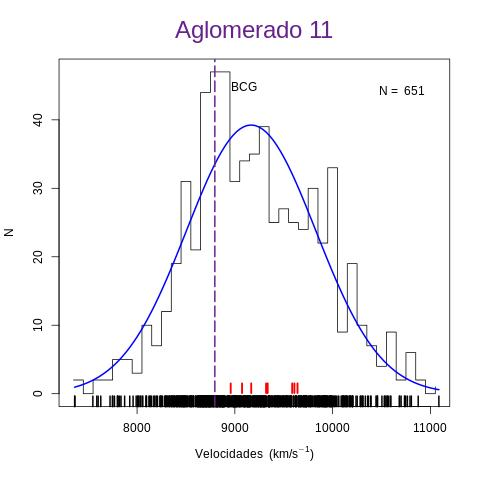
\includegraphics[scale=.23]{04-figuras/selec20/dist11}}
\subfloat{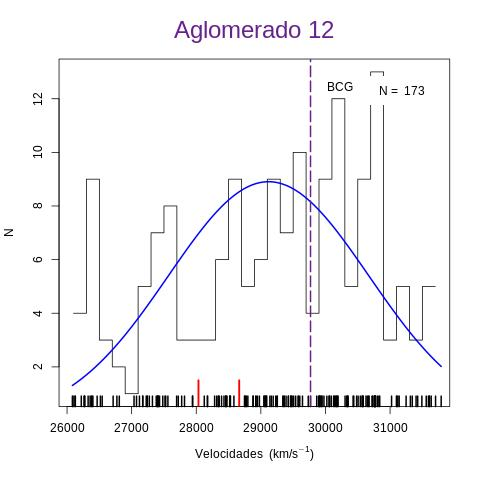
\includegraphics[scale=.23]{04-figuras/selec20/dist12}}\hfill
\subfloat{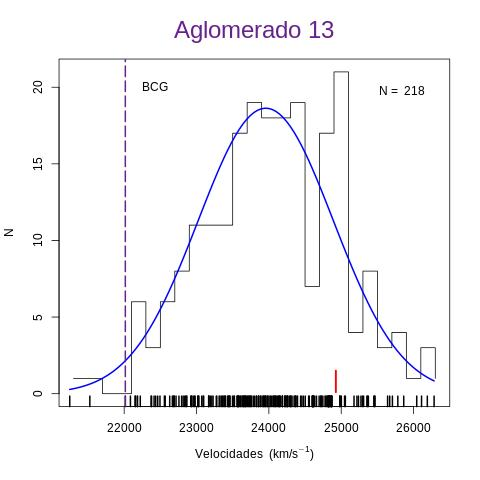
\includegraphics[scale=.23]{04-figuras/selec20/dist13}}
\subfloat{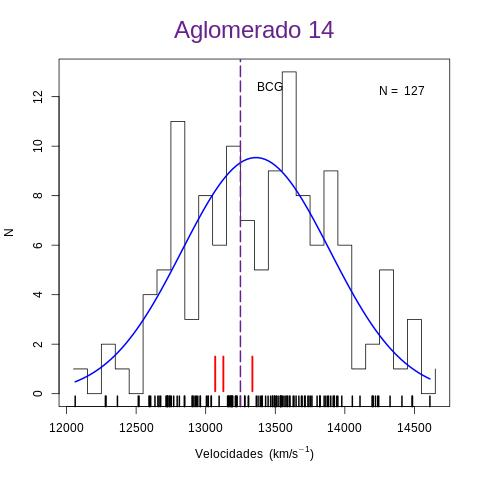
\includegraphics[scale=.23]{04-figuras/selec20/dist14}}
\subfloat{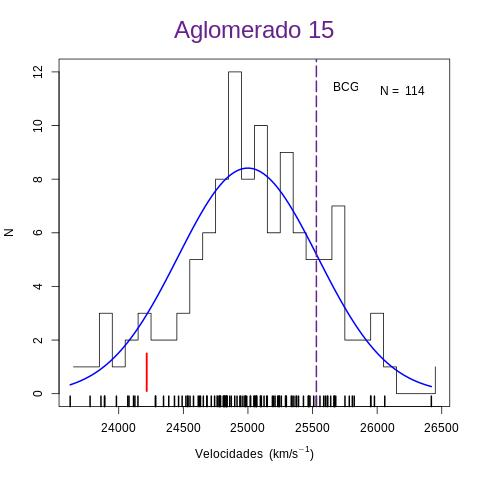
\includegraphics[scale=.23]{04-figuras/selec20/dist15}}
\subfloat{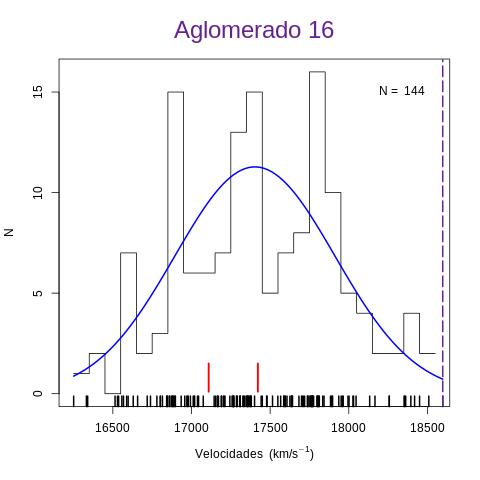
\includegraphics[scale=.23]{04-figuras/selec20/dist16}}\hfill
\subfloat{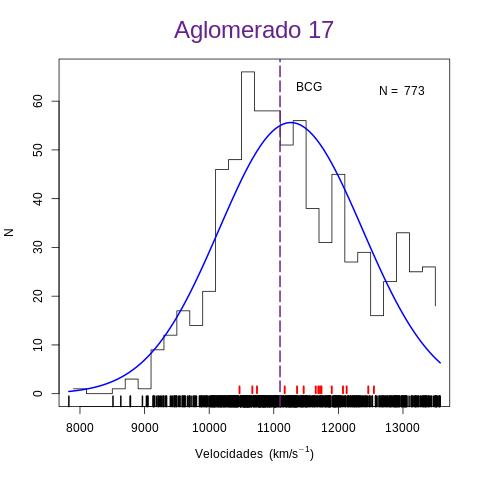
\includegraphics[scale=.23]{04-figuras/selec20/dist17}}
\subfloat{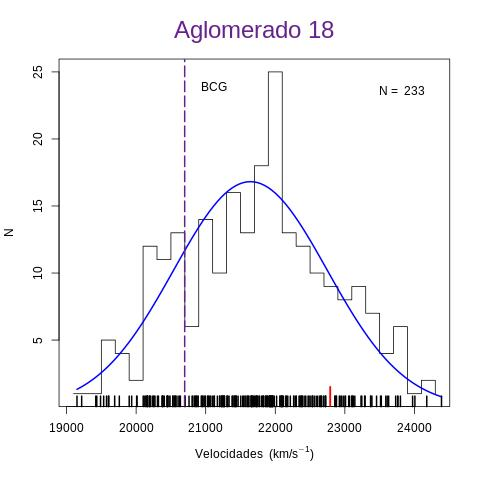
\includegraphics[scale=.23]{04-figuras/selec20/dist18}}
\subfloat{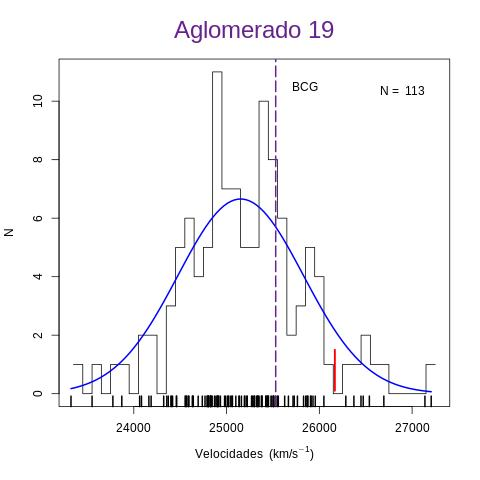
\includegraphics[scale=.23]{04-figuras/selec20/dist19}}
\subfloat{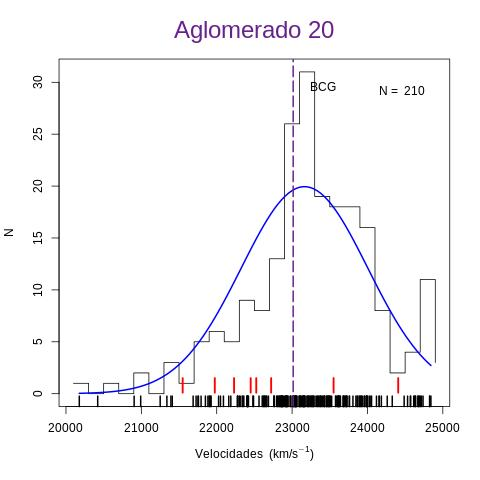
\includegraphics[scale=.23]{04-figuras/selec20/dist20}}
\caption{Histograma Distribuição de Velocidade e Análise de Gaps.}
\label{fig:fig4}%
\end{figure}


\begin{figure}[H] %h or !htbp
\vspace{-2pt}
\begin{center}
\subfloat{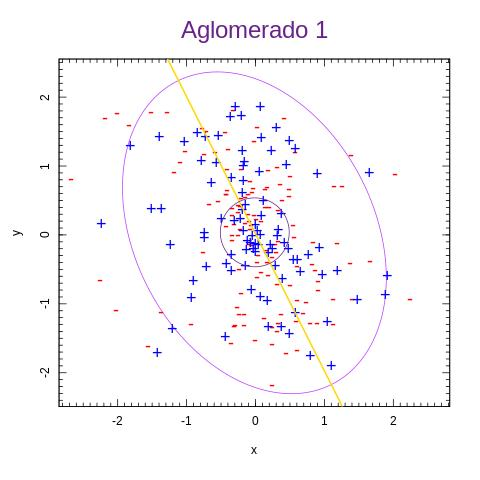
\includegraphics[scale=.23]{04-figuras/selec20/eixo01}}
\subfloat{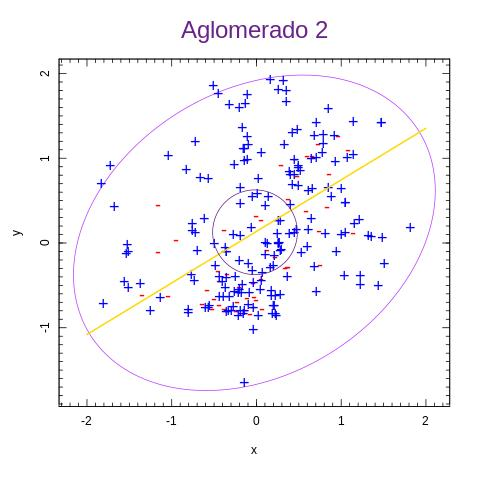
\includegraphics[scale=.23]{04-figuras/selec20/eixo02}}
\subfloat{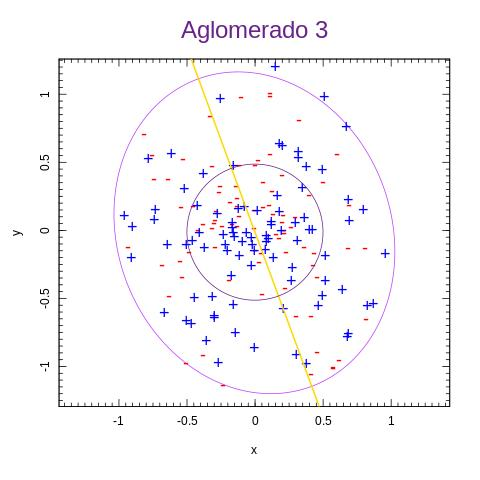
\includegraphics[scale=.23]{04-figuras/selec20/eixo03}}
\subfloat{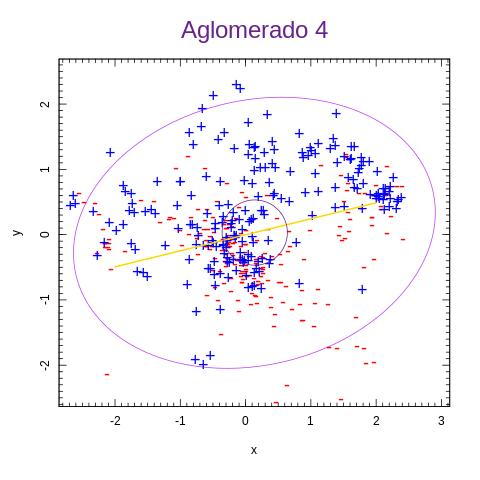
\includegraphics[scale=.23]{04-figuras/selec20/eixo04}}\hfill
\subfloat{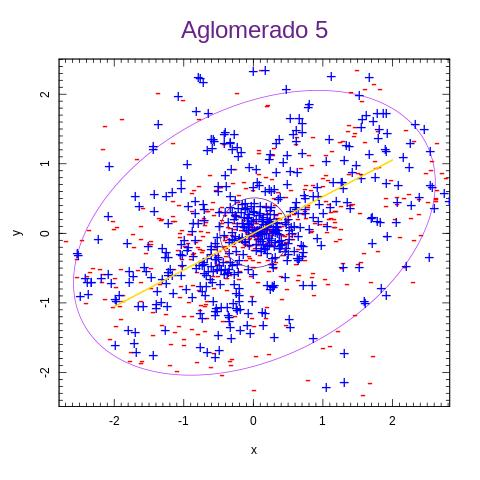
\includegraphics[scale=.23 ]{04-figuras/selec20/eixo05}}
\subfloat{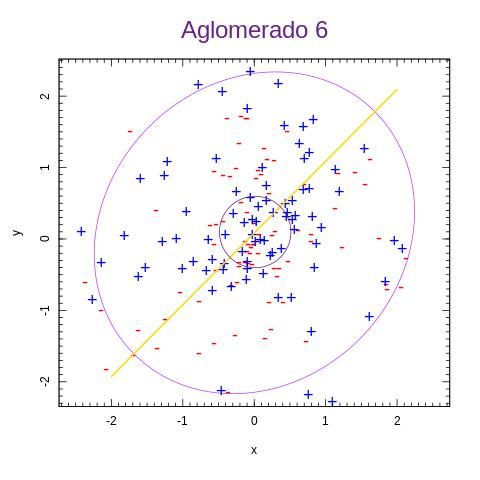
\includegraphics[scale=.23 ]{04-figuras/selec20/eixo06}}
\subfloat{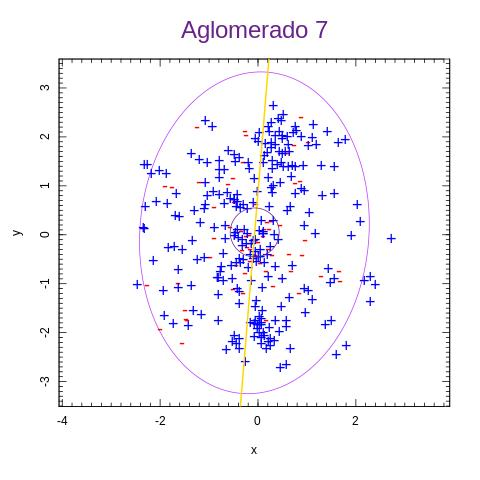
\includegraphics[scale=.23 ]{04-figuras/selec20/eixo07}}
\subfloat{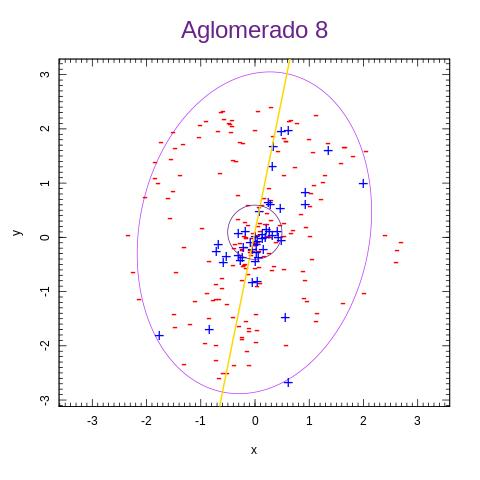
\includegraphics[scale=.23 ]{04-figuras/selec20/eixo08}}\hfill
\subfloat{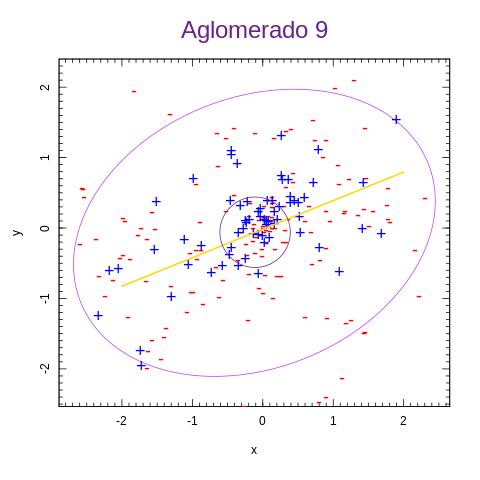
\includegraphics[scale=.23 ]{04-figuras/selec20/eixo09}}
\subfloat{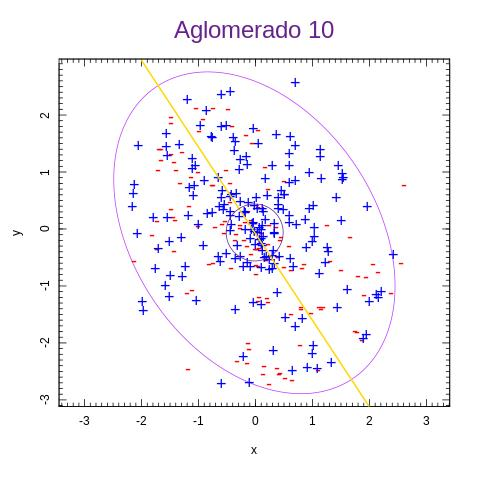
\includegraphics[scale=.23 ]{04-figuras/selec20/eixo10}}
\subfloat{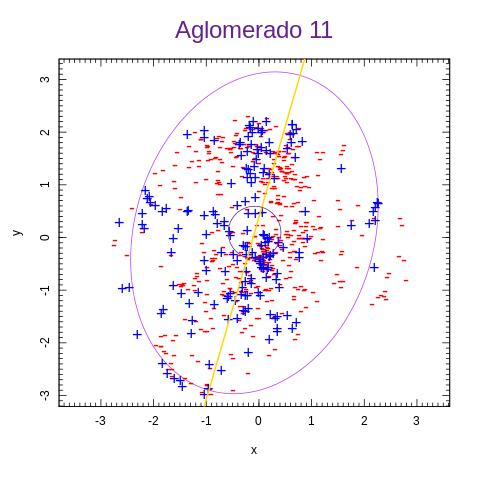
\includegraphics[scale=.23 ]{04-figuras/selec20/eixo11}}
\subfloat{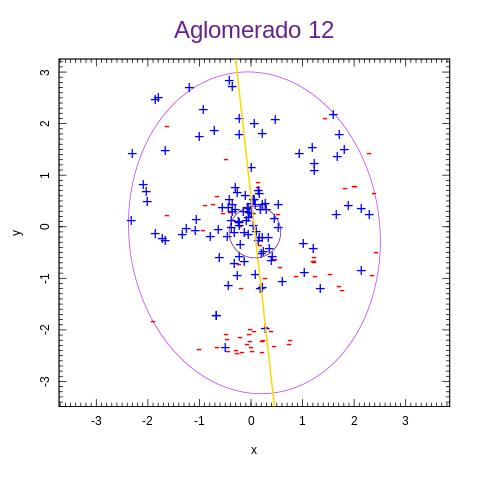
\includegraphics[scale=.23 ]{04-figuras/selec20/eixo12}}\hfill
\subfloat{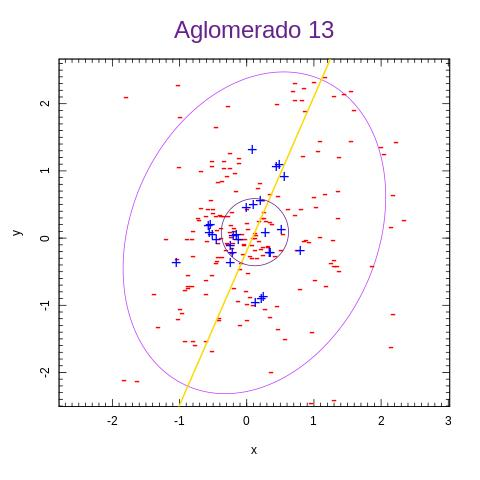
\includegraphics[scale=.23 ]{04-figuras/selec20/eixo13}}
\subfloat{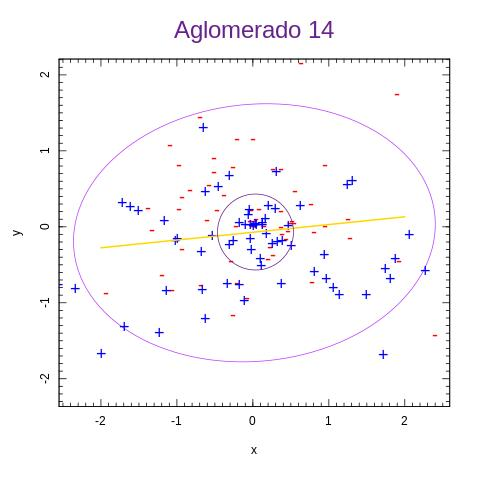
\includegraphics[scale=.23 ]{04-figuras/selec20/eixo14}}
\subfloat{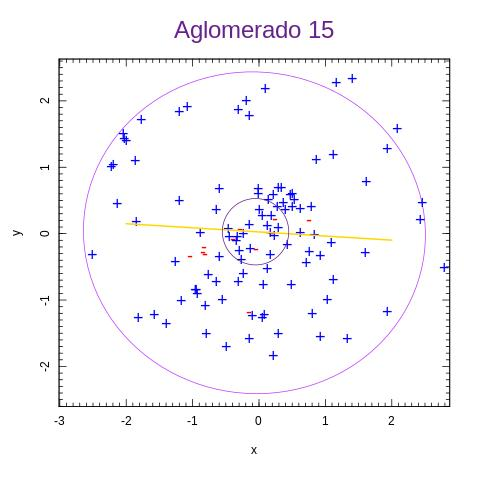
\includegraphics[scale=.23 ]{04-figuras/selec20/eixo15}}
\subfloat{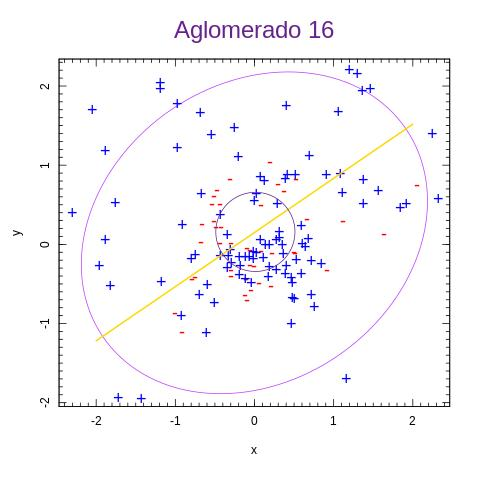
\includegraphics[scale=.23 ]{04-figuras/selec20/eixo16}}\hfill
\subfloat{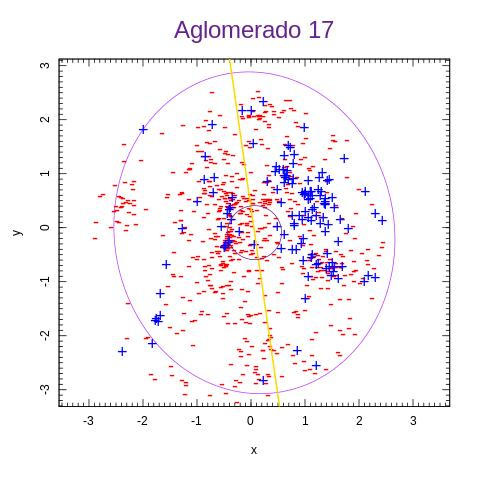
\includegraphics[scale=.23 ]{04-figuras/selec20/eixo17}}
\subfloat{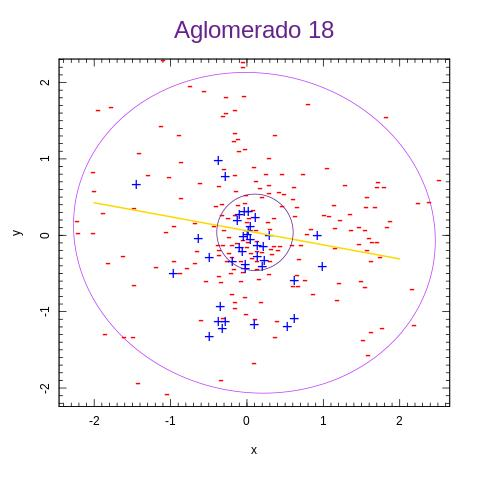
\includegraphics[scale=.23 ]{04-figuras/selec20/eixo18}}
\subfloat{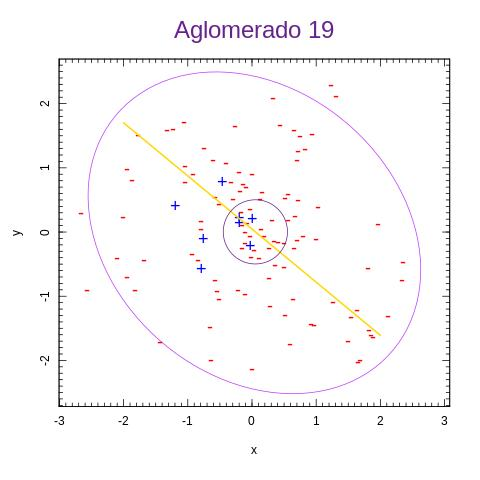
\includegraphics[scale=.23 ]{04-figuras/selec20/eixo19}}
\subfloat{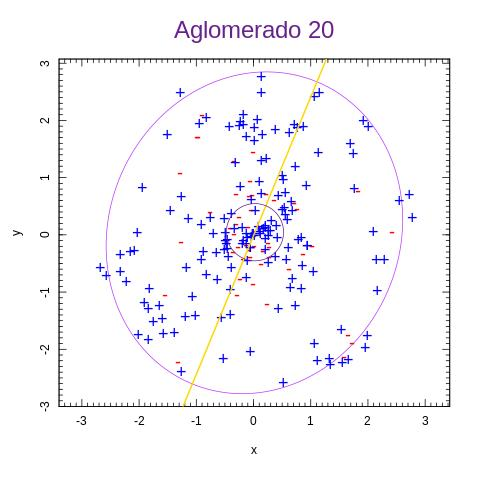
\includegraphics[scale=.23 ]{04-figuras/selec20/eixo20}}
\caption{Ajuste da elipse e eixo principal da distribuição projetada no plano do céu.}
\label{fig5}%
\end{center}
\end{figure}


\begin{figure}[H] %h or !htbp
\vspace{-2pt}
\begin{center}
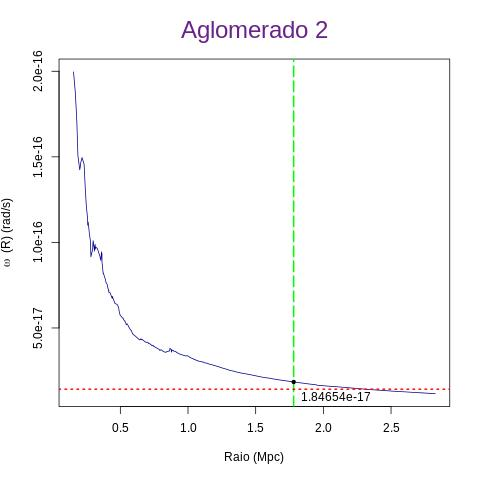
\includegraphics[scale=.3]{04-figuras/selec20/perfil02}%
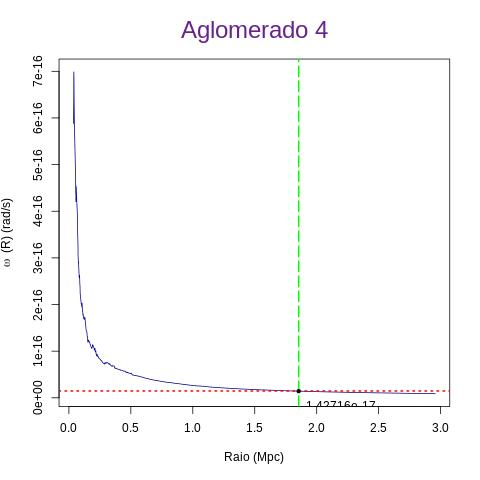
\includegraphics[scale=.3]{04-figuras/selec20/perfil04}
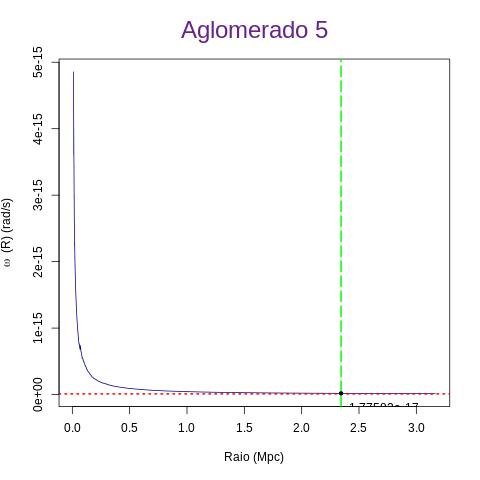
\includegraphics[scale=.3]{04-figuras/selec20/perfil05}
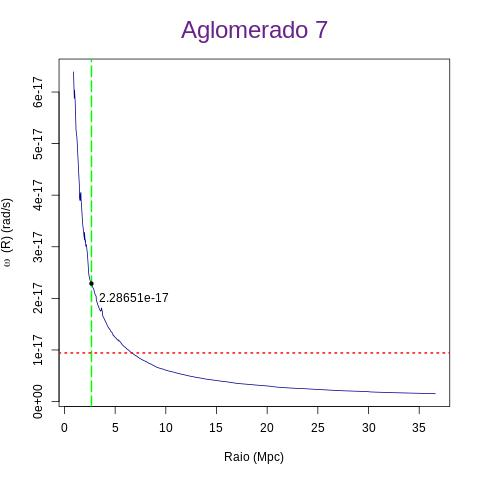
\includegraphics[scale=.3]{04-figuras/selec20/perfil07}\hfill
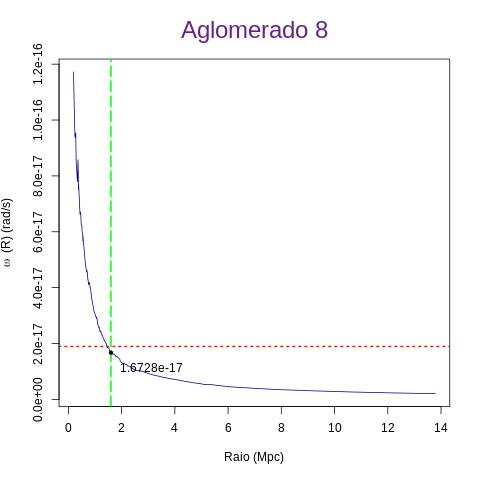
\includegraphics[scale=.3]{04-figuras/selec20/perfil08}
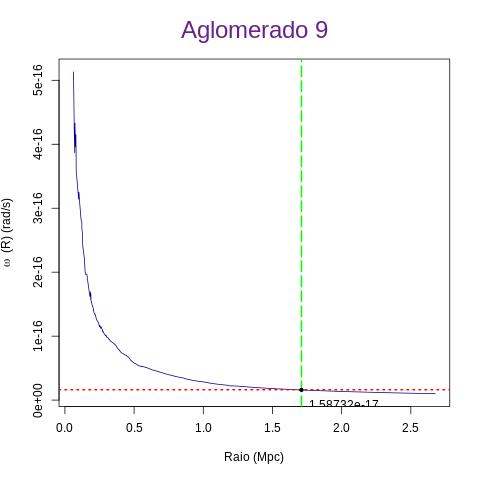
\includegraphics[scale=.3]{04-figuras/selec20/perfil09}
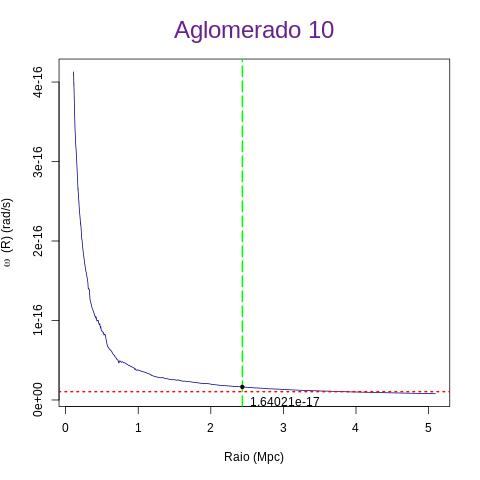
\includegraphics[scale=.3]{04-figuras/selec20/perfil10}
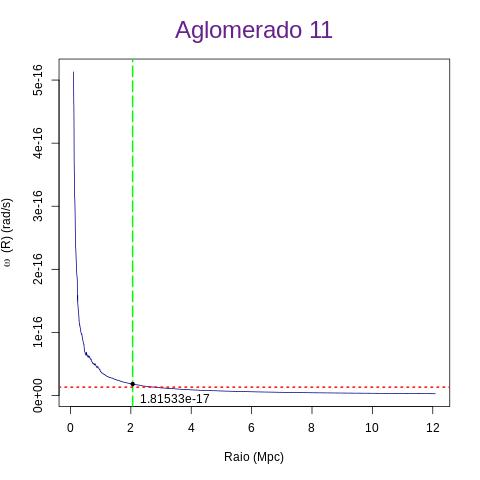
\includegraphics[scale=.3]{04-figuras/selec20/perfil11}\hfill
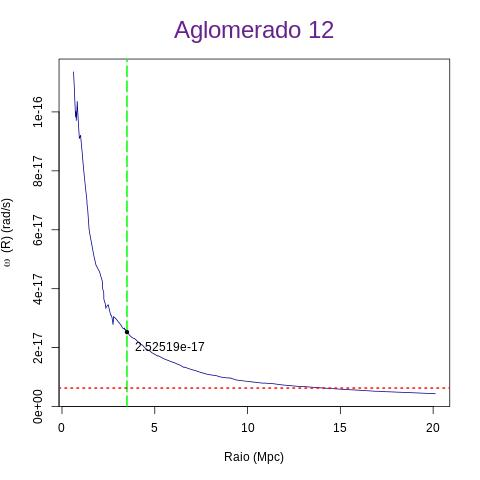
\includegraphics[scale=.3]{04-figuras/selec20/perfil12}
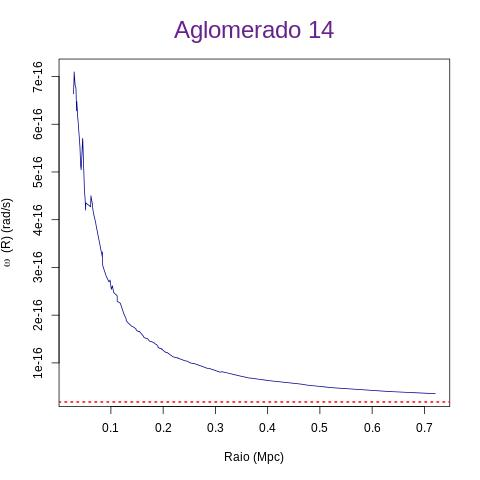
\includegraphics[scale=.3]{04-figuras/selec20/perfil14}
\includegraphics[scale=.3]{04-figuras/selec20/perfil15}
\includegraphics[scale=.3]{04-figuras/selec20/perfil16}\hfill
\includegraphics[scale=.3]{04-figuras/selec20/perfil17}
\includegraphics[scale=.3]{04-figuras/selec20/perfil18}
\caption{Perfil da velocidade de rotação.}
\label{fig6}%
\end{center}
\end{figure}


\chapter{Apêndice B: Resultados Catálogo NoSOCS}
\label{chap:apendicenosocs}


\end{apendicesenv}